\documentclass[a4paper,indent]{paper}
\usepackage{tikz}
\usepackage{microtype}
\usepackage{inputenc}
\usepackage{rotating}
\usepackage{fullpage}
\usepackage{caption}
\usepackage{tikz}
\usepackage{tikz-timing}
\usepackage{mdframed}
\usepackage{fourier} % for /danger
\usepackage{amsmath}

\usetikzlibrary{arrows, shapes.gates.logic.US, calc}

\title{Auger Radio Digitizer}
\subtitle{Software and interfaces}
\author{%
  Sjoerd T. Timmer (s.timmer@astro.ru.nl)\\
  Roel Jordans (r.jordans@astro.ru.nl)}
\date{}


%\newmdenv[linecolor=orange,backgroundcolor=orange!10]{warning}

\newenvironment{warning}
{\par\begin{mdframed}[linewidth=2pt,linecolor=orange,backgroundcolor=orange!10]%
    \begin{list}{}{\leftmargin=0mm}\item[\bf\danger{}~~Warning: ]}
  {\end{list}\end{mdframed}\par}

\begin{document}
\maketitle{}
\begin{abstract}
  This document describes the internal firmware architecture of the Auger Radio Digitizer (RD) module and the external interface to the UUB board.  
\end{abstract}

\clearpage

\section{Physical interface}
The Auger RD module is connected to the UUB with a 25 pin D-sub connector. At the time of writing this connects to a JST B24B connector on the UUB but this will soon be replaced with a SAMTEC STMM-112-01-S-D connector. The 25 pins contain 8 LVDS data signals and multiple power (+24V) and ground points.
Of the eight data signals, four are dedicated to data transfers and four are dedicated to the housekeeping interface:%

%\noindent%
\begin{tabular}{llllllll}
  %\shortstack{UUB\\fpga\\pin} &%
  \shortstack{UUB\\schema\\name} &%
  \shortstack{JST B24B\\(old connector)} &%
  \shortstack{SAMTEC\\STMM-112\\-01-S-D(new)} &%
  \shortstack{D-sub\\pin} &%
  \shortstack{RD schema\\name} &%
  \shortstack{RD fpga\\pin} &%
  \shortstack{pin\\function}
  \\\hline
  EXTn\_P\_D1 & 1   & 2  & 1  & LVDS\_0+  & L4 & SPI MOSI\\
  EXTn\_N\_D1 & 2   & 1  & 14 & LVDS\_0-  & L5 &  \\
  EXTn\_P\_D0 & 3   & 4  & 2  & LVDS\_1+  & J3 & SPI CLK \\
  EXTn\_N\_D0 & 4   & 3  & 15 & LVDS\_1-  & K3 &  \\
  GND         & 5   & 6  & 3  & GND       &    &  \\
  24V         & 6   & 5  & 16 & 24V       &    &  \\
  EXTn\_P\_D2 & 7   & 8  & 4  & LVDS\_2+  & K2 & DATA 0 \\
  EXTn\_N\_D2 & 8   & 7  & 17 & LVDS\_2-  & J1 &  \\
  EXTn\_P\_D4 & 9   & 10 & 5  & LVDS\_3+  & M4 & DATA 1 \\
  EXTn\_N\_D4 & 10  & 9  & 18 & LVDS\_3-  & N5 &  \\
  GND         & 11  & 12 & 6  & GND       &    &  \\
  24V         & 12  & 11 & 19 & 24V       &    &  \\
  EXTn\_P\_D3 & 13  & 14 & 7  & LVDS\_4+  & G2 & DATA CLK \\
  EXTn\_N\_D3 & 14  & 13 & 20 & LVDS\_4-  & F1 &  \\
  EXTn\_P\_D5 & 15  & 16 & 8  & LVDS\_5+  & N4 & SPI CE \\
  EXTn\_N\_D5 & 16  & 15 & 21 & LVDS\_5-  & P5 &  \\
  GND         & 17  & 18 & 9  & GND       &    &  \\
  24V         & 18  & 17 & 22 & 24V       &    &  \\
  EXTn\_P\_D6 & 19  & 20 & 10 & LVDS\_6+  & P3 & TRIGGER \\
  EXTn\_N\_D6 & 20  & 19 & 23 & LVDS\_6-  & P4 &  \\
  EXTn\_P\_D7 & 21  & 22 & 11 & LVDS\_7+  & N2 & SPI MISO \\
  EXTn\_N\_D7 & 22  & 21 & 24 & LVDS\_7-  & M1 &  \\
  GND         & 23  & 24 & 12 & GND       &    &  \\
  24V         & 24  & 23 & 25 & 24V       &    &  \\
              &     &    & 13 & GND or NC &    &  \\
\end{tabular}
\captionof{table}{Pin mapping}

\begin{center}
  \begin{minipage}[b]{0.2\textwidth}
    \centering
    \includegraphics[height=4cm]{img/images-000.png}
  \end{minipage}
  \begin{minipage}[b]{0.5\textwidth}
    \centering
    \includegraphics[height=6cm]{img/images-002.png}
  \end{minipage}
  \begin{minipage}[b]{0.2\textwidth}
    \centering
    \includegraphics[height=4cm]{img/images-004.png}
  \end{minipage}
  \begin{minipage}[t]{0.2\textwidth}
    \centering
    \captionof{figure}{D-sub}
  \end{minipage}
  \begin{minipage}[t]{0.5\textwidth}
    \centering
    \captionof{figure}{JST B24B}
  \end{minipage}
  \begin{minipage}[t]{0.2\textwidth}
    \centering
    \captionof{figure}{SAMTEC STMM-112-01-S-D}
  \end{minipage}
\end{center}



\section{Software interface}
The Auger RD module has two separate interfaces. One fast interface to capture radio traces, and one slower SPI interface for housekeeping. 

\subsection{Radio data}
The Auger RD module samples 12-bit data from 2 channels at 250 Msamples/s into a circular buffer.
It does so continuously until it sees a high level on the trigger input. When the trigger is received the RD will continue to write the post-trigger samples to the buffer.
The number of pre-trigger and post-trigger samples can be configured using the housekeeping/SPI interface and defaults to 1024/1024 at boot.
See Section \ref{sec:trigger_offset} for details about how to change the trigger offset. The total buffer always contains 2048 samples.

When the post-trigger samples have been recorded, the transfer is automatically initiated.
See Figure~\ref{fig:datatransferstart}~and~\ref{fig:datatransferfinish} for an overview of the data transfer. 
The transfer is clocked from the RD at 60MHz. The clock is silent outside the transmission windows.
The transmission starts with a preamble consisting of three rising clock edges.
After the preamble, the 2048 samples are transmitted. Data for the two channels is separately transmitted on the two data lines.
Each sample is shifted out, most significant bit first, followed by a parity bit (odd parity). Finally eleven trailing clock cycles are transmitted.

\begin{center}
  \begin{minipage}[b]{\textwidth}
    \centering
    %\includegraphics[width=\textwidth]{img/data-transfer-start.pdf}
    \begin{tikztimingtable}[timing/wscale=1.2]
      clk     & HHLCCCCCCCCCCCCCCCCCCCCCCCCCCCCCCCCCCCCCCCCCCCC \\ 
      data[0] & UUUUUUUUDDDDDDDDDDDDDDDDDDDDDDDD{Sample 0 Channel 0 [11:0]}DD{parity}DDDDDDDDDDDDD{Sample 1 Channel 0 [11:0]} \\
      data[1] & UUUUUUUUDDDDDDDDDDDDDDDDDDDDDDDD{Sample 0 Channel 1 [11:0]}DD{parity}DDDDDDDDDDDDD{Sample 1 Channel 1 [11:0]} \\
    \end{tikztimingtable}
    \captionof{figure}{Start of data transfer has 3 leading clock edges. Data is stable at rising edges. Parity bit follows data.}\label{fig:datatransferstart}
  \end{minipage}\vspace{\baselineskip}
  \begin{minipage}[b]{\textwidth}
    \centering
    %\includegraphics[width=\textwidth]{img/data-transfer-finish.pdf}
    \begin{tikztimingtable}[timing/wscale=1.2]
      clk     & CCCCCCCCCCCCCCCCCCCCCCCCCCCCCCCCCCCCCCCCHHHHHHH \\ 
      data[0] & DDDDDDDDDDDDDDDD{Sample 2047 Channel 0 [11:0]}DD{parity}UUUUUUUUUUUUUUUUUUUUUUUUUUUUU \\
      data[1] & DDDDDDDDDDDDDDDD{Sample 2047 Channel 1 [11:0]}DD{parity}UUUUUUUUUUUUUUUUUUUUUUUUUUUUU \\
    \end{tikztimingtable}
    
    \captionof{figure}{End of data transfer has 11 trailing rising edges.}\label{fig:datatransferfinish}
  \end{minipage}
\end{center}

There is negligeable delay between the registration of the last sample and the start of the transmission and between the end of the transmission and the registration of the first sample for the next trace.

During the transmission and during the recording of the pre-trigger samples the value of the trigger input is ignored.



\subsection{Jitter and latency}\label{sec:latency}
Data is transferred from an ADC (ADS4229) to an FPGA (Lattice ECP5 LFE5U-12F) over 12 LVDS pairs. The data transfer is DDR (dual data rate) which means that the even bits are transferred on the rising edges of the 250 MHz clock and the odd bits on the falling edges. In the FPGA the DDR data is decoded and further processed at 125 MHz. I.e., samples are processed four at a time (two samples each from two channels). This means that triggers are also registered at the 125 MHz clock and that the RD inherently incurs a 1 sample jitter on the location of the trigger.  

Using the trigger offset feature of the SPI housekeeping interface, the location of the data window relative to the trigger can be configured. By default the location is set to 1024. I.e. the center of the window. However, the trigger signal is synchronized to the 125 MHz clock domain using two registers. This results in two clock cycles delay (i.e. four samples).

The ADC is also subject to 16 clock cycles latency (at 250 MHz). In total there are therefore 1020 or 1021 samples before the trigger and 1027 or 1028 samples after the trigger.

\begin{warning}
  An experiment is planned but not yet executed to verify if the 12 sample delay is correctly calculated and --in particular-- if the jitter of 1 additional clock cycle is applied correctly the the mentioned figures.
\end{warning}

As noted, this can offset using the SPI interface. 

\begin{center}
  \includegraphics[width=\textwidth]{img/rd_timing.pdf}
  \captionof{figure}{Timing of RD capture}\label{fig:rd_timing}
\end{center}

\subsection{SPI housekeeping interface}

The SPI interface exposes several features including firmware updates, science ADC re-configuration, trigger injection, gpio access and readout of operating temperatures, voltages and currents. 
These are internally bridged in a demuxer. The first eight bits of every spi transaction are captured by the demuxer. The remainder of the transaction is forwarded transparently to the sub-system in question.

\begin{center}
  \begin{tikztimingtable}
    clk               & CCCCCCCCCCCCCCCCCCCCCCCCCCCCCCCCCCCC \\
    ce in             & HHLLLLLLLLLLLLLLLLLLLLLLLLLLLLLLLLHH \\
    mosi              & UUDDDDDDDDDDDDDDDD{address, e.g. 0x06}DDDDDDDDDDDDDDDD{forwarded data}UU \\
    \ldots            & \\
    ce to system 0x05 & HHHHHHHHHHHHHHHHHHHHHHHHHHHHHHHHHHHH \\
    ce to system 0x06 & HHHHHHHHHHHHHHHHHHLLLLLLLLLLLLLLLLHH \\
    ce to system 0x07 & HHHHHHHHHHHHHHHHHHHHHHHHHHHHHHHHHHHH \\
    \ldots            & \\
  \end{tikztimingtable}
  \captionof{figure}{SPI demuxer example}
\end{center}


\subsubsection{SPI mode and speed}
The SPI interface was tested upto 12 MHz. It is known that all sub-systems can also reach that speed.
The external interface operates with CPOL=1 and CPHA=1 (spi mode 3) at all times. The ADS4229 science adc operates in mode 2 but the responsible sub-system block handles the translation. 


\subsubsection{Housekeeping sub-systems}
The following subsystems are currently implemented:
\paragraph{GPIO (address 0x01)}
Eight gpio pins are available in the RD board. All pins are configured as outputs. The GPIO sub-systems allows writing and reading of the output buffer. Each transaction exists of a single byte command, optionally followed by a data byte in case of a write command.

The supported commands are:
\begin{center}
  \begin{tabular}{|l|l|}
    \hline
    command & code \\
    \hline
    read & 0x00 \\
    write & 0x01 \\
    set bits (gpio = gpio or data) & 0x02 \\
    clear bits (gpio = gpio and not data) & 0x03 \\
    reset to default & 0x04 \\
    \hline
  \end{tabular}
  \captionof{table}{GPIO commands}
\end{center}

\begin{center}
  \begin{tikztimingtable}
    clk  & HHCCCCCCCCCCCCCCCCCCCCCCCCCCCCCCCCCCCCCCCCCCCCCCCCHH \\
    ce   & HHLLLLLLLLLLLLLLLLLLLLLLLLLLLLLLLLLLLLLLLLLLLLLLLLHH \\
    mosi & UUDDDDDDDDDDDDDDDD{0x01 (select GPIO)}DDDDDDDDDDDDDDDD{0x00 (GPIO read)}UUUUUUUUUUUUUUUUUU \\
    miso & UUUUUUUUUUUUUUUUUUUUUUUUUUUUUUUUUUDDDDDDDDDDDDDDDD{0x42 (for example)}UU \\
  \end{tikztimingtable}
  \vspace{\baselineskip}\\
  \begin{tikztimingtable}
    clk  & HHCCCCCCCCCCCCCCCCCCCCCCCCCCCCCCCCCCCCCCCCCCCCCCCCHH \\
    ce   & HHLLLLLLLLLLLLLLLLLLLLLLLLLLLLLLLLLLLLLLLLLLLLLLLLHH \\
    mosi & UUDDDDDDDDDDDDDDDD{0x01 (select GPIO)}DDDDDDDDDDDDDDDD{0x01 (GPIO write)}DDDDDDDDDDDDDDDD{0x00 (for example)}UU \\
    miso & UUUUUUUUUUUUUUUUUUUUUUUUUUUUUUUUUUDDDDDDDDDDDDDDDD{0x42 (old data)}UU \\
  \end{tikztimingtable}
  \captionof{figure}{Example GPIO read and write. The output register contains the data 0x42 and is written to 0x00.}
\end{center}


\paragraph{Program flash pass-through (address 0x02)}
Transactions to address 0x02 are forwarded transparently to the SPI flash chip.
Refer to the SST26VF032B documentation for details.

\begin{center}
  \begin{tikztimingtable}[timing/wscale=0.6]
    clk      & HHCCCCCCCCCCCCCCCCCCCCCCCCCCCCCCCCCCCCCCCCCCCCCCCCCCCCCCCCCCCCCCCCCCCCCCCCCCCCCCCCHH \\
    uub ce   & HHLLLLLLLLLLLLLLLLLLLLLLLLLLLLLLLLLLLLLLLLLLLLLLLLLLLLLLLLLLLLLLLLLLLLLLLLLLLLLLLLHH \\
    flash ce & HHHHHHHHHHHHHHHHHHLLLLLLLLLLLLLLLLLLLLLLLLLLLLLLLLLLLLLLLLLLLLLLLLLLLLLLLLLLLLLLLLHH \\
    mosi     & UUDDDDDDDDDDDDDDDD{0x02 (select spi flash)}DDDDDDDDDDDDDDDD{0x9F (read id)}UUUUUUUUUUUUUUUUUUUUUUUUUUUUUUUUUUUUUUUUUUUUUUUUUU \\
    miso     & UUUUUUUUUUUUUUUUUUUUUUUUUUUUUUUUUUDDDDDDDDDDDDDDDD{0xBF}DDDDDDDDDDDDDDDD{0x26}DDDDDDDDDDDDDDDD{0x42}UU\\
  \end{tikztimingtable}
  \captionof{figure}{Example SST26VF032B JEDEC-ID readout.}
\end{center}



\paragraph{Science adc pass-through (address 0x03)}
The science ADC has a SPI configuration interface. The ADS4229 expects SPI mode 2 (cpol=1, cpha=0) but also works in spi mode 1 (cpol=0, cpha=1) which is achieved by inverting the clock signal from the uub interface.

\begin{center}
  \begin{tikztimingtable}[timing/wscale=1]
    uub spi clk & HHCCCCCCCCCCCCCCCCCCCCCCCCCCCCCCCCCCCCCCCCCCCCCCCCHH \\
    uub spi ce  & HHLLLLLLLLLLLLLLLLLLLLLLLLLLLLLLLLLLLLLLLLLLLLLLLLHH \\
    mosi        & UUDDDDDDDDDDDDDDDD{0x03 (select ADS4229 adc)}DDDDDDDDDDDDDDDD{0x25 (gain register)}DDDDDDDDDDDDDDDD{0x40 gain setting}UU \\
    adc spi ce  & HHHHHHHHHHHHHHHHHHLLLLLLLLLLLLLLLLLLLLLLLLLLLLLLLLHH \\
    adc spi clk & LLLLLLLLLLLLLLLLLLCCCCCCCCCCCCCCCCCCCCCCCCCCCCCCCCLL \\
  \end{tikztimingtable}
  \captionof{figure}{Example ADS4229 transaction. This sets the channel A gain (config register address 0x25) to 2dB .}
\end{center}




\paragraph{ADS1015 current and voltage sensors (address 0x04)}
\begin{warning}
  The exact control of the ADS1015 and Si7060 is under debate and subject to change.
\end{warning}

The ADS1015 is a four port I2C ADC which is wired to measure the voltage and the current on both LNA channels. This can be used to determine if the LNA is properly connected and working as expected.

Whenever a trigger is received via either the trigger input or via the housekeeping trigger injection, the controller for this I2C chip will execute a fixed sequence of I2C commands and store the conversion result in a register. The register can be read via SPI and contains eight bytes:

\begin{center}
  \begin{tabular}{|l|l|}
    \hline
    Register address & contents \\
    \hline
    0x00 & bits [11:4] of ADC channel 0 (current N/S bias)\\
    0x01 & bits [3:0]  of ADC channel 0, followed by four zeroes\\
    0x02 & bits [11:4] of ADC channel 1 (voltage N/S bias)\\
    0x03 & bits [3:0]  of ADC channel 1, followed by four zeroes \\
    0x04 & bits [11:4] of ADC channel 2 (current E/W bias)\\
    0x05 & bits [3:0]  of ADC channel 2, followed by four zeroes \\
    0x06 & bits [11:4] of ADC channel 3 (voltage E/W bias)\\
    0x07 & bits [3:0]  of ADC channel 3, followed by four zeroes \\
    \hline
  \end{tabular}
  \captionof{table}{ADS1015 register layout}
\end{center}

Upon receiving a trigger, the RD delays the readout of the I2C devices until all science data has been written to the internal buffer. This is done to avoid polution of the spectrum, even though the 400 kHz communication is not believed to be powerful enough to be picked up by our antenna. After completing the buffer but before initiating the science data transfer the four conversions are started. Because the ADS1015 makes one ADC conversion at a time the samples are not made in parallel but sequentially. Due to the maximum sampling frequency (3300 SPS) the RD has to stall for 315 ns after each conversion. 
All four conversions take 2.16 ms in total to complete. If another trigger is received in that time it does not cause another readout but rather assumes that the previously read values are still correct.

The ADS1015 has a PGA. All conversions are made with the $FSR=\pm4.096 V$ setting. I.e. $MSB = 2 mV$.

To read a byte from the register simply write the address of that register and read the data on the next byte. The next address can already be written during the read and therefore the whole register can efficiently be read in nine bytes (excluding the subsystem address byte).

\begin{center}
  \begin{tikztimingtable}[timing/wscale=0.8]
    clk  & HHCCCCCCCCCCCCCCCCCCCCCCCCCCCCCCCCCCCCCCCCCCCCCCCCCCCCCCCCCCCCCCCCHH \\
    ce   & HHLLLLLLLLLLLLLLLLLLLLLLLLLLLLLLLLLLLLLLLLLLLLLLLLLLLLLLLLLLLLLLLLHH \\
    mosi & UUDDDDDDDDDDDDDDDD{0x04 (select ADS1015)}DDDDDDDDDDDDDDDD{0x04}DDDDDDDDDDDDDDDD{0x05}UUUUUUUUUUUUUUUUUU \\
    miso & UUUUUUUUUUUUUUUUUUUUUUUUUUUUUUUUUUDDDDDDDDDDDDDDDD{$I_{E/W}[11:4]$}DDDDDDDD{$I_{E/W}[3:0]$}DDDDDDDD{0000}UU \\
  \end{tikztimingtable}
  \captionof{figure}{Example ADS1015 register readout for the E/W bias current.}
\end{center}


\paragraph{SI7060 temperature sensor (address 0x05)}
\begin{warning}
  The exact control of the ADS1015 and Si7060 is under debate and subject to change.
\end{warning}

The Si7060 is a I2C temperature sensor which measures the temperature inside the RD enclosure.

Whenever a trigger is received via either the trigger input or via the housekeeping trigger injection, the controller for this I2C chip will execute a fixed sequence of I2C commands and store the conversion result in a register. The register can be read via SPI and contains two bytes:

\begin{center}
  \begin{tabular}{|l|l|}
    \hline
    Register address & contents \\
    \hline
    0x00 & Dspsigm of Si7060 (one status bit and data bits [14:8])\\
    0x01 & Dspsigl of Si7060 (data bits [7:0])\\
    \hline
  \end{tabular}
  \captionof{table}{ADS1015 register layout}
\end{center}

Upon receiving a trigger, the RD delays the readout of the I2C devices until all science data has been written to the internal buffer. This is done to avoid polution of the spectrum, even though the 400 kHz communication is not believed to be powerful enough to be picked up by our antenna. After completing the buffer but before initiating the science data transfer the temperature conversion is started.
The entire readout including conversion takes 0.2475 ms in total to complete. If another trigger is received in that time it does not cause another readout but rather assumes that the previously read values are still correct.

The raw 15-bit data is calculated as:
$$
D =  \text{Dspsigm}[6:0] < < 8 + \text{Dspsigl}[7:0]
$$

The temperature can be calculated as follows:
$$
T (^\circ{}C) = 55 + (D - 16384) / 160
$$



To read a byte from the register simply write the address of that register and read the data on the next byte. The next address can already be written during the read and therefore the whole register can efficiently be read in nine bytes (excluding the subsystem address byte).

\begin{center}
  \begin{tikztimingtable}[timing/wscale=0.8]
    clk  & HHCCCCCCCCCCCCCCCCCCCCCCCCCCCCCCCCCCCCCCCCCCCCCCCCCCCCCCCCCCCCCCCCHH \\
    ce   & HHLLLLLLLLLLLLLLLLLLLLLLLLLLLLLLLLLLLLLLLLLLLLLLLLLLLLLLLLLLLLLLLLHH \\
    mosi & UUDDDDDDDDDDDDDDDD{0x05 (select Si7060)}DDDDDDDDDDDDDDDD{0x00}DDDDDDDDDDDDDDDD{0x01}UUUUUUUUUUUUUUUUUU \\
    miso & UUUUUUUUUUUUUUUUUUUUUUUUUUUUUUUUUUDDDDDDDDDDDDDDDD{Dspsigm}DDDDDDDDDDDDDDDD{Dspsigl}UU \\
  \end{tikztimingtable}
  \captionof{figure}{Example Si7060 temperature readout.}
\end{center}




\paragraph{Trigger injection (address 0x06)}
Triggers can be injected into the RD if no physical trigger is present. This is useful for debugging. The inverted CE of this submodule is OR'ed with the external trigger input. It is not necessary to send any data for the trigger to work.
\begin{center}
  \begin{tikztimingtable}[timing/wscale=1]
    clk    & HHCCCCCCCCCCCCCCCCHH \\
    ce     & HHLLLLLLLLLLLLLLLLHH \\
    mosi   & UUDDDDDDDDDDDDDDDD{0x06 (internal trigger)}UU \\
    trig\_int & HHHHHHHHHHHHHHHHHLHH \\
  \end{tikztimingtable}
  \captionof{figure}{Example transaction to inject an internal trigger.}
\end{center}
\begin{center}
  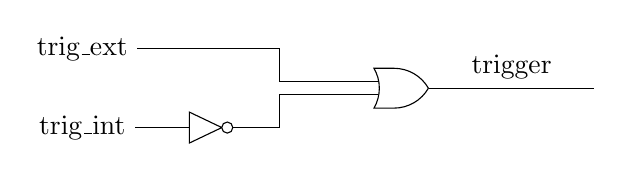
\begin{tikzpicture}
    \node (te) at (0, 1) {trig\_ext};
    \node (ti) at (0, 0) {trig\_int};
    \node[not gate US, draw] at ($(ti) + (1.5, 0)$) (notti) {};
    \node[or gate US, draw, rotate=0, logic gate inputs=nn] at ($(notti) + (2.5, 0.5)$) (teornotti) {};
    \draw (ti) -- (notti.input);
    \draw (te) -- (2.5,1) |- (teornotti.input 1);
    \draw (notti.output) -- (2.5,0) |- (teornotti.input 2);
    \draw (teornotti.output) -- node[above]{trigger} ($(teornotti) + (2.5, 0)$);
  \end{tikzpicture}
  \captionof{figure}{Internal wiring of internal and external trigger.}
\end{center}




\paragraph{Version info (address 0x07)}
This subsystem will always return a 1-byte version code.
The currently known version codes are:
\begin{center}
  \begin{tabular}{|l|l|}
    \hline
    Code & Description \\
    \hline
    0x00 & legacy (version info not implemented) \\
    0x01, 0x02 & used during development \\
    0x03 & version shipped with RDv3 units for the Malargue engineering array in November 2019\\
    \hline
  \end{tabular}
\end{center}



\paragraph{Start offset configuration(address 0x08)}
The position of the trigger within the data window can be configured.
This start offset is set to 1024 (mid window) on power up but can be changed using this interface.
The value is set by writing two bytes to this subsystem. Only the lower eleven bits are used. The upper 5 bits are ignored.
The written number represents the position in the data trace where the trigger will be located. Note that the actual trigger appears at a slightly different position due to latency in the ADC and in the RD. Refer to Figure~\ref{fig:rd_timing} for details.
\begin{center}
  \begin{tikztimingtable}[timing/wscale=1]
    clk  & HHCCCCCCCCCCCCCCCCCCCCCCCCCCCCCCCCCCCCCCCCCCCCCCCCHH \\
    ce   & HHLLLLLLLLLLLLLLLLLLLLLLLLLLLLLLLLLLLLLLLLLLLLLLLLHH \\
    mosi & UUDDDDDDDDDDDDDDDD{0x08 (select offset reg)}UUUUUUUUUUDDDDDD{offset[11:8]}DDDDDDDDDDDDDDDD{offset[7:0]}UU \\
  \end{tikztimingtable}
  \captionof{figure}{Example Si7060 temperature readout.}
\end{center}


\subsubsection{Boot time and boot sequence}
After power is applied the FPGA loads its configuration from the SST26VF032B SPI flash.
After the user code is running the RD executes a hard-coded initialization sequence on the SPI interface, as if the UUB had sent the following commands:

\begin{center}
  \begin{tabular}{|l|l|}
    \hline
    SPI commands & Description \\
    \hline
    \texttt{0x03 0x00 0x02} & ADS4229 software reset \\
    \texttt{0x03 0x29 0x00} & re-assert default configuration \\
    \texttt{0x03 0x41 0x00} & re-assert default configuration \\
    \texttt{0x03 0x03 0x03} & enable high-performance mode \\
    \texttt{0x03 0xF2 0x00} & disable low speed mode (already off by default)\\
    \texttt{0x03 0xEF 0x00} & disable low speed mode (already off by default)\\
    \texttt{0x03 0x41 0x00} & cmos mode off (already off by default)\\
    \texttt{0x03 0x02 0x40} & enable high performance mode \\
    \texttt{0x03 0xD5 0x18} & enable high performance mode \\
    \texttt{0x03 0xD7 0x0C} & enable high performance mode \\
    \texttt{0x03 0xDB 0x20} & enable high performance mode \\
    \texttt{0x08 0x04 0x00} & set start offset to 1024 \\
    \hline
  \end{tabular}
  \captionof{table}{RD initialization sequence. }
  
\end{center}

This initialization sequences takes approximately 170 us. During this time the SPI lines from the UUB are inhibited and the MISO line will remain silent.




\section{Developers Guide/Architecture}
\subsection{General architecture}
\subsubsection{SPI demux}

\subsubsection{Boot sequence injection}


\subsection{Housekeeping subsystems}

\subsubsection{Program flash (0x02)}

\subsubsection{Science ADC (0x03)}

\subsubsection{Current and voltage monitoring (0x04)}

\subsubsection{Temperature sensor (0x05)}

\subsubsection{Trigger injection (0x06)}

\subsubsection{Firmware version register (0x07)}

\subsubsection{Trigger offset register (0x08)}

\section{Architecture of RD firmware}

\subsubsection{Write Controller}
%The write controller is responsible for enabling and disabling writes to the circular buffer.
%It listens in on the address counter ($i\_curr\_address$) and controls (besides the write enable ($o\_write\_enable$)) the start ($o\_trigger\_done$) and start offset ($o\_start\_addr$) of the Readout Controller.
%
%A configurable start offset ($i\_start\_offset$) determines how many samples are stored before the trigger.
%In the current instantiation the address width is eleven bits so there are 2048 samples and therefore $2048 - i\_start\_offset$ samples after the trigger.
%
%
%The Write Controller needs to be enabled with a pulse on the $i\_arm$ input.
%After this pulse the Write Controller will enable writes within 2 clock cycles.
%
%The ADC driver outputs 2 samples in each clock cycle (for each channel, so 4 in total at each clock cycle).
%Therefore the Write Controller should wait for at least
%$$
%\left\lceil\frac{i\_start\_offset}{2}\right\rceil
%$$
%clock cycles  before accepting triggers.
%
%After the trigger is first seen high, the Write Controller should keep $o\_write\_enable$ high for exactly
%$$
%\left\lceil\frac{2048 - i\_start\_offset}{2}\right\rceil
%$$
%clock cycles. At that time $o\_write\_enable$ has to be asserted low and $o\_trigger\_done$ should be asserted high. At that time $o\_start\_addr$ has to be set to the address at which the data starts:
%$$
%i\_curr\_addr - i\_start\_offset \pmod{2048}
%$$
%This condition should hold until the next pulse on the $i\_arm$ signal.
%
%
%A start offset of 0 (or 1) is considered invalid but anything in the closed interval $[1, 2047]$ should work.
%





\end{document}